%!TEX root = lec06_transactions.tex



%%%%%%%%%%%%%%%%%%%%%%%%%

%
% -------------------------------------
%
\begin{frame}{Simplified DBMS architecture}

\begin{center}
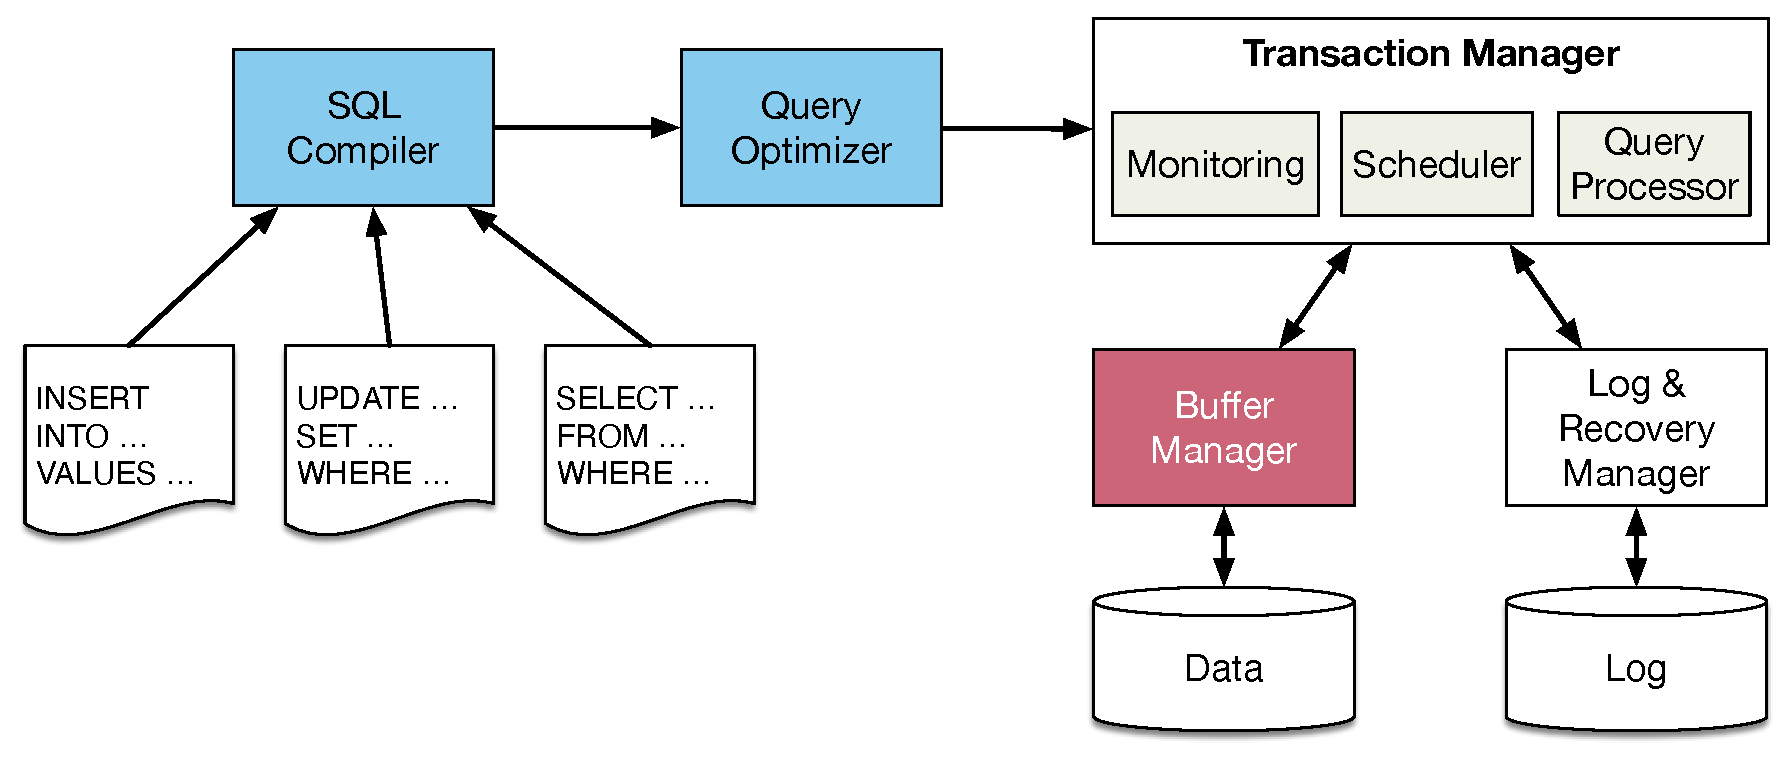
\includegraphics[width=0.8\textwidth]{../lec00_intro/figures/dbms_architecture.eps}
\end{center}

These notes look into the theory and algorithms to ensure the correct and concurrent execution of queries and updates.

First, we consider the execution of transactions in isolation. Then we look at the concurrent execution of transactions.
\end{frame}


%
% -------------------------------------
%
\begin{frame}

\begin{BOX}{What is a transaction?}
A sequence of operations to fulfill a user request that may involve reading and/or writing data, and computing values from the data:\\
- queries are ``read-only'' transactions that do not modify the database;\\
- SQL \lstinline[style=SQL]{INSERT}, \lstinline[style=SQL]{DELETE}, and \lstinline[style=SQL]{UPDATE} commands typically read some data, compute new values, and write (or overwrite) some data back to the database.
\end{BOX}

\vskip1em

Every transaction is \textbf{logically independent} of other transactions.

We say a transaction:\\
- \textbf{COMMITS} if it executes in its entirety; or\\
- \textbf{ABORTS} if it cannot be executed in its entirety by the DBMS.
\end{frame}


%
% -------------------------------------
%
\begin{frame}[fragile]

Every update command (received from the command line interface or via an API call from an application program) is \emph{implicitly} wrapped in a transaction.

\vskip1em

\begin{center}
\begin{minipage}{0.75\textwidth}
\begin{lstlisting}[style=SQL]
> INSERT INTO R VALUES (2),(1);
\end{lstlisting}
\end{minipage}
\end{center}

is executed as

\vskip0.4em

\begin{center}
\begin{minipage}{0.75\textwidth}
\lstset{style=SQL,%
  keywords=[1]{INSERT,INTO,VALUES},
  keywords=[4]{BEGIN,TRANSACTION,COMMIT},keywordstyle=[4]\ttfamily\bfseries\color{exampleColor}}
\begin{lstlisting}[style=SQL]
BEGIN TRANSACTION;
INSERT INTO R VALUES (2),(1);
COMMIT;
\end{lstlisting}
\end{minipage}
\end{center}
\end{frame}


%
% -------------------------------------
%
\begin{frame}{ACID Transactions}

Most relational systems implement the ACID transaction model:

\begin{itemize}
	\item{\highlight{A}TOMICITY}: every transaction must either execute in its entirety or not at all

	\item{\highlight{C}ONSISTENCY}: every transaction must leave the database in a consistent state

	\item{\highlight{I}SOLATION}: no transaction can interfere with the execution of another transaction

	\item{\highlight{D}URABILITY}: if a transaction \textbf{COMMITS}, all its changes to the database must become permanent
\end{itemize}
\end{frame}


%
% -------------------------------------
%
\begin{frame}[fragile]{Atomicity}

Most transactions involve many read/write/compute operations and take some time to execute. Atomicity means that the DBMS cannot execute just \emph{some} of the operations in a transaction. 

In other words, the DBMS must do one of:
\begin{itemize}[-,topsep=-0.5em]
\item \underline{Execute \textbf{all operations} in a transaction} and \lstinline[style=SQL]{COMMIT} it, making its effects permanent.
\item \underline{Leave the database unchanged} and \lstinline[style=SQL]{ABORT} the transaction.
\end{itemize}

\vskip0.5em

\begin{BOX}{Why would an operation fail?}
There are many reasons; e.g., attempting to update the database in a way that violates a constraint, reaching a timeout limit for user input, etc.
\end{BOX}
\end{frame}


%
% -------------------------------------
%
\begin{frame}{Consistency}

Recall that a database instance is \textbf{consistent} if (and only if) it satisfies \underline{all constraints} defined in its schema:
\begin{itemize}[-,topsep=-0.5em,noitemsep]
  \item Domain, \lstinline[style=SQL]{UNIQUE}, and \lstinline[style=SQL]{NOT NULL} constraints.
  \item Primary and foreign key constraints.
  \item Complex constraints defined using triggers.
\end{itemize}

\vskip1em

Domain, unique, and key constraints are checked first, for each tuple inserted, deleted or modified by the transaction.

Next, the DBMS executes all triggers associated with the tables being modified by the transaction. 

If no violations or exceptions are detected, the transaction is allowed to commit.
\end{frame}

%
% ----------------------
%

\newsavebox\SQLiteAutoROLLBACKexample
\begin{lrbox}{\SQLiteAutoROLLBACKexample}
\begin{lstlisting}[style=SQL,numbers=left,frame=leftline]
CREATE TABLE T(a INT, PRIMARY KEY a);
BEGIN TRANSACTION;
    INSERT INTO T VALUES (1);
    INSERT INTO T VALUES (2);
    INSERT INTO T VALUES (1);
    INSERT INTO T VALUES (3);
COMMIT;
\end{lstlisting}
\end{lrbox}


\begin{frame}[fragile]{What exactly happens when some statements fail?}

\begin{columns}[onlytextwidth]
\begin{column}{0.475\textwidth}
What happens when some statements in a transaction are successful while others fail \textbf{depends on the DBMS}.
\end{column}
\begin{column}{0.425\textwidth}
\scalebox{0.75}{\usebox\SQLiteAutoROLLBACKexample}
\end{column}
\end{columns}

\vskip1em

In the code above, most systems will automatically rollback\footnote{Rollback means reverting the database objects to their original values.} the transaction, leaving the table empty.

SQLite, on the other hand, \textbf{does not} automatically rollback updates\footnote{\url{https://sqlite.org/lang_transaction.html}}. Instead, it leaves it to the application to decide what to do upon the constraint violation in line 5.

\end{frame}

%
% -------------------------------------
%
\begin{frame}{Isolation}

In the strictest sense, isolation means that every transaction must execute as if it was the only transaction in the system.

In other words, isolation means that once a transaction starts executing, no other transaction should be allowed to modify the data that will be used by that transaction.

\vskip0.5em

\begin{BOX}{Isolation and Concurrency are conflicting goals}
Ensuring isolation may prevent opportunities for concurrency.

\vskip1em

With SQL, the programmer can choose among different levels of isolation, and thus fine tune of the concurrency/isolation trade-off.
\end{BOX}

\end{frame}


%
% -------------------------------------
%
\begin{frame}{Durability}

Durability means that the effects of a transaction become permanent if (and only if) it commits.

\vskip0.5em

Durability is enforced by:
\begin{itemize}[-,topsep=-0.5em,noitemsep]
 \item Ensuring dirty buffers and the log are written to storage.
 \item Using reliable storage (redundant storage, RAID system, etc.).
\end{itemize}
 
\vskip1.5em

\begin{BOX}{Crash Recovery}
In the event of a crash (e.g., power failure), the DBMS must be able to restore the database to reflect all changes made by all transactions that committed before the crash. 

This is done by processing the entries in the log.
\end{BOX}
\end{frame}


%
% ------------------------------------- RUNNING EXAMPLE
%


\newsavebox{\exampleA}
\savebox{\exampleA}{%
\scriptsize%
\begin{tabular}{@{}rc | l }
  & \multicolumn{2}{l}{\textbf{Holder}}\\
  \cline{2-3}
  & \cellcolor{Gray}\textbf{id} & \cellcolor{Gray}\textbf{Name} \\
  \cline{2-3}
  & 1234 & Hurit \\
  \cline{2-3}
  & 7564 & Nuttah \\
  \cline{2-3}
  & 7890 & Kimi \\
  \cline{2-3}
\end{tabular}
}

\newsavebox{\exampleB}
\savebox{\exampleB}{%
\scriptsize%
\begin{tabular}{@{}r l | l | l }
& \multicolumn{3}{l}{\textbf{Account}}\\
\cline{2-4}
& \cellcolor{Gray}\textbf{holder} & \cellcolor{Gray}\textbf{type} & \cellcolor{Gray}\textbf{balance} \\
\cline{2-4}
$t_1$ & 7564 & checking & 75\\
\cline{2-4}
& 1234 & savings & 50 \\
\cline{2-4}
$t_2$ & 7564 & investment & 40\\
\cline{2-4}
\end{tabular}
}

\newsavebox\UPDATEexample
\begin{lrbox}{\UPDATEexample}
\begin{lstlisting}[style=SQL,linewidth=0.75\textwidth,frame=single]
BEGIN TRANSACTION; -- transfer between accounts

UPDATE Account SET balance = balance - 20
WHERE holder = 7564 AND type = 'checking';

UPDATE Account SET balance = balance + 20
WHERE holder = 7564 AND type = 'investment';

COMMIT;
\end{lstlisting}
\end{lrbox}


%
% -------------------------------------
%


